\documentclass[12pt]{article}

\usepackage{sbc-template}

\usepackage{graphicx,url}

\usepackage[brazil]{babel}
\usepackage[utf8]{inputenc}
\usepackage[T1]{fontenc}
\usepackage{mathtools}
\usepackage{amsmath}
\usepackage{listings}

\usepackage{todonotes}
\usepackage{xargs}
\newcommandx{\change}[2][1=]{\todo[linecolor=red,backgroundcolor=red!25,bordercolor=red,#1]{#2}}

\lstset{ %
frame=single
}


\sloppy

\title{\libname: Uma biblioteca de lógica \textit{fuzzy} direcionada à GPUs}

% Edevaldo Braga dos Santos
% Giovane de Oliveira Torres
% Guilherme Pereira Paim
% Renan Zafalon da Silva
% Vitor Alano de Ataides

\author{Edevaldo Braga dos Santos\inst{1}, Giovane de Oliveira Torres\inst{1}, Guilherme Pereira Paim\inst{1},\\ Renan Zafalon da Silva\inst{1}, Vitor Alano de Ataides\inst{1}, Maurício Lima Pilla\inst{1}}

\address{Universidade Federal de Pelotas \\
Pelotas, RS - Brasil\\
  \email{\{edevaldo.santos,gdotorres,gppaim,renan.zafalon,vaataides,pilla\}} \\
  \texttt{\begin{footnotesize}@inf.ufpel.edu.br\end{footnotesize}}
}

\begin{document}

\newcommand{\libname}{CudaFuzzy}

\maketitle

%\begin{abstract}

%Abstract aqui.

%\end{abstract}

\begin{resumo}

O trabalho desenvolvido foi implementar uma biblioteca de lógica fuzzy voltada às GPUs, de maneira a aproveitar o paralelismo disponível neste tipo de arquiteturas. Algumas operações foram implementadas em suas versões sequenciais e paralelas, a fim de extrair os resultados deste artigo. Os resultados obtidos mostram que as operações que efetuaram mais cálculos matemáticos tendem a ter melhor desempenho, o que é potencializado incrementando o número de operações que são executadas.

\end{resumo}

\section{Introdução}
\label{sec:introducao}

% Logica fuzzy: colocar onde? %

	Existem diversos casos onde classes de objetos não pertencem totalmente a um conjunto. Baseado nisso, Zadeh definiu a teoria dos conjuntos \textit{fuzzy}~\cite{zadeh:65}, que visa tratar problemas de imprecisão ao classificar dados no mundo real. Os conjuntos \textit{fuzzy} possuem aplicações em sistemas de controle e de suporte a decisão, onde a descrição do problema não é feita de forma precisa~\cite{weber:03}.
	
	Utilizando os conhecimentos provenientes dos conjuntos \textit{fuzzy}, se tem a base para a utilização da lógica \textit{fuzzy}, sendo construída a partir da lógica proposicional. Com isso, os operadores foram definidos a partir dos já estabelecidos na lógica clássica, com a adição de outros, para fins práticos~\cite{tanscheit:04}. Uma característica interessante, que diferencia a lógica tradicional da \textit{fuzzy}, é que na primeira os valores que utilizados atendem à condição de serem verdadeiros ou falsos (0 ou 1). Já na segunda, trabalha-se com conjuntos \textit{fuzzy}, os quais podem assumir um valor que pertence ao intervalo $[0, 1]$. Isso permite que um conjunto \textit{fuzzy} possa ser representado por uma infinidade de valores~\cite{klir:95}.	
	
% GPU %

	Com a finalidade de obter computação com bom desempenho, se torna importante o uso dos vários núcleos de processamento, disponibilizados nos sistemas de computação atuais, visando um melhor aproveitamento do paralelismo do sistema computacional. Neste contexto, encaixam-se as GPUs (\textit{Graphical Processor Units}), que são componentes com alto poder de paralelismo~\cite{sengupta:07}. Porém, é importante ressaltar que as GPUs são reservadas a obter bom desempenho com aplicações que possuem determinadas características~\cite{owens:08}, que incluem: (i) Requisitos computacionais excessivos, (ii) Paralelismo nas aplicações e (iii) maior importância do \textit{throughput} em detrimento da latência. Destacam-se ainda alguns exemplos práticos, bem-sucedidos, que utilizam CUDA:
Através do uso do poder computacional de CUDA, para análise do fluxo de tráfego aéreo, foi possível reduzir o tempo de análise do tráfego aéreo nacional de dez minutos para três segundos. Outro exemplo relevante é o ganho de desempenho em simulações moleculares NAMD (dinâmica molecular em nanoescala), nelas o ganho de desempenho foi possível graças às arquiteturas paralelas das GPUs~\cite{nvidia:15}.

	Tendo sido discutidos estes conceitos, o objetivo deste trabalho é descrever uma biblioteca de lógica \textit{fuzzy} voltada para GPUs, a fim de verificar a forma como pode ser efetuada uma implementação que consiga extrair paralelismo deste tipo de arquiteturas. Com isto, fez-se a implementação da biblioteca, e então também desenvolveu-se uma versão sequencial para obter os principais resultados, comparando as duas implementações.
	
	Os resultados mostrados neste trabalham mostram que as operações em geral obtiveram algum tipo de \textit{speedup} na implementação paralela sobre a sequencial. Os melhores resultados encontraram-se nas operações que envolviam mais complexidade em cálculos matemáticos e com maiores tamanhos de \textit{array} considerados. Esta última ocorrida devido à maneira que a GPU gerencia o paralelismo, visto que é necessário bastante quantidade de operações para que haja eficiência ao executar as computações.
	
	O restante deste artigo está dividido da seguinte maneira: A Seção~\ref{sec:logfuzzy} fala sobre a lógica fuzzy, que é a base para a construção deste trabalho. Na Seção~\ref{sec:lib}, é descrita a implementação efetuada da biblioteca~\libname. A Seção~\ref{sec:metodologia} destina-se a explicar a metodologia empregada para a execução de testes na biblioteca. Na Seção~\ref{sec:resultados} são exibidos e discutidos os principais resultados obtidos por este trabalho, de onde se tiram as principais conclusões, observadas na Seção~\ref{sec:conclusoes}, a qual ainda mostra possíveis trabalhos futuros. Por fim, na Seção~\ref{sec:trabalhos} faz-se uma breve discussão sobre os trabalhos que relacionam-se ao escopo deste artigo.

\section{Lógica \textit{Fuzzy}}
\label{sec:logfuzzy}

A lógica \textit{fuzzy} foi criada com base na teoria de conjuntos \textit{fuzzy}. A principal ideia da lógica \textit{fuzzy} é aumentar a representação de valores, não restrigindo-se somente aos valores 0 (falso) e 1 (verdadeiro). Um valor na lógica \textit{fuzzy} é representado por um número real que está entre os números 0 e 1 -- e esse, representa o grau de pertinência do valor dentro de um conjunto \textit{fuzzy}~\cite{boclin:06}. A teoria dos conjuntos \textit{fuzzy} foi criada com o propósito de oferecer ferramentas matemáticas que visam solucionar problemas que possuam algumas das seguintes características~\cite{falcao:02}: Incerteza, informações vagas e ambiguidade.

%Lógica fuzzy foi criada com base na teoria de conjuntos Fuzzy, a ideia principal de fuzzy é a seguinte: Um valor é verdadeiro (grau 1) ou falsos (grau 0), sendo que o grau pode variar de 0 a 1. A teoria do conjunto fuzzy foi inventada com o objetivo de oferecer ferramentas matemáticas para solucionar problemas imprecisos ou vagos. Dentre as inúmeras aplicações com lógica fuzzy, o projeto IMMO-RATE, é bastante interessante, pois ele permite análise de sustentabilidade em imóveis, considerando questões chaves específicas que utilizam a lógica fuzzy.

\subsection{Operadores \textit{Fuzzy}}
Conjuntos são definidos por uma condição específica que define se um conjunto pertence ou não a outro. Para exemplificar os operadores em \textit{fuzzy}, logo abaixo foram utilizados conjuntos A e B.
Os mais comuns em conjuntos \textit{fuzzy} são: 

\begin{itemize}
	\item União: (A\begin{math} \cup \end{math} B = x | x \begin{math}\in \end{math} A \begin{math}\vee \end{math} x \begin{math}\in \end{math} B)
	\item Intersecção: (A \begin{math} \cap \end{math} B = x | x \begin{math}\in \end{math}A \begin{math}\wedge \end{math} x \begin{math}\in \end{math} B)
\end{itemize}

Além dos operadores em conjuntos, os operadores aritméticos são fundamentais para a matemática \textit{fuzzy}. Os operadores adição e subtração são mais fáceis de manipular, já os procedimentos de multiplicação e divisão são mais complexos. Novamente utilizando como exemplo dois conjuntos A e B, as principais operações aritméticas são:

\begin{itemize}
	\item Adição - 
\begin{math} [{a_1},{a_3}] (+) [{b_1},{b_3}]= [{a_1 + b_1,a_3 + b_3}]  \end{math}
	\item Subtração - \begin{math} [{a_1},{a_3}] (-) [{b_1},{b_3}] = [{a_1 - b_1,a_3 - b_3}]  \end{math}
	\item Multiplicação - 
\begin{math} [{a_1},{a_3}] (\bullet) [{b_1},{b_3}]= [{a_1 \bullet b_1,a_3 \bullet b_3}]  \end{math}
	\item Divisão - 
\begin{math} [{a_1},{a_3}] (/) [{b_1},{b_3}]= [{a_1 / b_1,a_3 / b_3}]  \end{math} 
\end{itemize}

\section{\libname}
\label{sec:lib}

	\libname~é o nome dado à biblioteca de lógica \textit{fuzzy} desenvolvida neste trabalho, voltada a GPUs. Para o seu desenvolvimento, a biblioteca criada teve a necessidade de incluir vários operadores, para trabalhar sobre os conjuntos \textit{fuzzy}. Foram escolhidas operações básicas~\cite{klir:95} para a implementação, sendo estas: duas operações AND ($\wedge$), duas operações OR ($\vee$) e três operações NOT ($\sim$). Na Figura~\ref{fig:fuzzyops} estão demonstradas as operações através dos operadores desenvolvidos.
	
\begin{figure}[!h]
\centering

\[ \begin{array}{ccc}
	AND1(x, y) & = & min(x, y) \\
	AND2(x, y) & = & x \times y \\
	OR1(x, y) & = & max(x, y) \\
	OR2(x, y) & = & (x + y) - (x \times y)\\
	NOT1(x) & = & 1 - x \\
	NOT2(x) & = & \sqrt{1-x^2} \\
	NOT3(x) & = & \sqrt[3]{1-x^3} \\
\end{array} \]
\caption{Operações implementadas na biblioteca~\libname}
\label{fig:fuzzyops}
\end{figure}

Os operadores foram implementados em C, utilizando-se a biblioteca CUDA, e foram desenvolvidos como funções que recebem como argumentos um ou dois valores do tipo \texttt{double} (um para operações \texttt{NOT}, e dois para operações \texttt{AND} e \texttt{OR}), sendo esses os operandos e retornando um valor do tipo \texttt{double}, o qual é o resultado da operação. Na Figura~\ref{fig:operation} está exemplificada a implementação da operação \texttt{NOT3}.

\begin{figure}[!h]
\centering
\lstinputlisting[language=C, firstline=43, lastline=45, otherkeywords={inline,device}]{d_FuzzyLogic.cu}
\caption{Código de implementação da operação de lógica \textit{fuzzy} NOT3}
\label{fig:operation}
\end{figure}

Porém, é importante observar que a implementação destes operadores, por si só, representa pouco do trabalho efetuado. Como as arquiteturas alvo para esta biblioteca são as GPUs, houve a necessidade de elaborar uma maneira de aproveitar o paralelismo disponível nestas arquiteturas. A estratégia abordada por este trabalho buscou agrupar conjuntos de operações de um mesmo tipo, em um \textit{array} de instruções. Com isso, surge a possibilidade de serem executadas múltiplas operações de lógica \textit{fuzzy} nos vários núcleos disponibilizados pela GPU. As operações são agrupadas em um mesmo tipo para serem executadas em paralelo devido à taxonomia destas arquiteturas, sendo elas consideradas SIMT (\textit{Single instruction multiple thread})~\cite{keckler:11}, Através da arquitetura SIMT uma mesma intrução é transmitida para várias unidades de execução, essa arquitetura é muito utilizada de forma a acelerar os processamentos nos sistemas de computação em alto desempenho, pois os núcleos dos processadores são grandes e os processadores SIMT executam uma grande quantidade de threads com um mesmo fluxo de instrução utilizando diferentes dados. \cite{lain:12}

Assim, as operações são feitas sobre uma função que leva o prefixo \texttt{Bulk}, o qual fará uma operação de lógica \textit{fuzzy} sobre um \textit{array} de operandos (Em caso de operações \texttt{BulkNOT}) ou sobre dois \textit{arrays} de operandos (Em caso de operações \texttt{BulkAND} e \texttt{BulkOR}). No caso de operações que trabalham com dois \textit{arrays}, essas serão efetuadas de maneira correspondente nos \textit{arrays}, i.e., o primeiro operando de um \textit{array} será combinado com o primeiro operando do outro \textit{array}, gerando assim uma computação parcial da operação, sendo esse o primeiro elemento do \textit{array} de resultado. Logo, quando a operação requer dois \textit{arrays} como entrada, os mesmos deverão conter o mesmo número de elementos. Na Figura~\ref{fig:bulkoperation} está representada uma computação parcial da operação \texttt{BulkAND1}.

\begin{figure}[!h]
\centering
\lstinputlisting[language=C, basicstyle=\scriptsize, firstline=187, lastline=194, otherkeywords={inline,device}]{d_BulkLogic.cu}
\caption{Código de implementação de uma única operação \texttt{BulkAND1}}
\label{fig:bulkoperation}
\end{figure}

	O código acima é a representação de uma operação efetuada entre o i-ésimo elemento de um \textit{array} com seu correspondente no segundo \textit{array}. O resultado desta operação gera o i-ésimo elemento do \textit{array}, o qual armazenará os resultados da operação \texttt{Bulk}. Ao final da execução de todas as operações que trabalham com cada elemento do \textit{array}, tem-se todos os resultados parciais no \textit{array} de resultado.

\section{Metodologia}
\label{sec:metodologia}

	A fim de extrair os resultados deste artigo, foi proposta uma metodologia. Após ser feita a implementação da biblioteca \libname, também foi construída uma versão sequencial da biblioteca a fim de comparar o ganho de desempenho paralelizando o código. Esta versão, em vez de executar em paralelo as operações dentro de um \textit{array}, é efetuado o cálculo de uma operação por vez.
	
	Foi feita então uma bateria de execuções para a geração dos resultados. Cada operação \texttt{Bulk} foi executada 30 vezes, em sua versão paralelizada usando GPU, bem como a versão sequencial. Em cada operação, foi testado diferentes tamanhos do \textit{array} usado nas operações \texttt{Bulk}, a fim de avaliar também o impacto que a variação neste atributo acarreta no desempenho da biblioteca. Os tamanhos de array considerados foram potências de 10, iniciando em 10 mil e terminando em 100 milhões de operações. Para extrair os tempos de execução e comparar as duas versões, obteve-se a média do total de execuções, além de efetuar o teste t de Student para comprovar a diferença estatística entre as médias.
	
	Os testes foram executados sobre uma máquina com processador Intel(R) Core(TM) i7-3630QM CPU 2.40GHz, com 24 GB de Memória RAM, utilizando o sistema operacional Linux Mint 17.3. A placa de vídeo empregada nas simulações foi a GeForce GTX 670, sendo usado a versão 7.5 do CUDA.
	
\section{Resultados e Discussão}	
\label{sec:resultados}

A principal contribuição do trabalho em termos de resultados está exibida no gráfico da Figura~\ref{fig:speedup}, onde é exibido o \textit{speedup} da implementação da biblioteca \libname~com a versão sequencial.

\begin{figure}[!h]
\centering
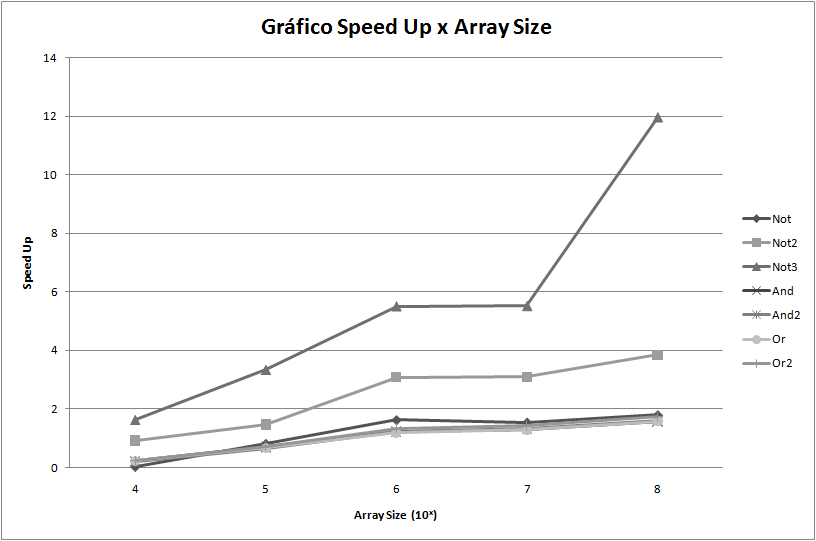
\includegraphics[scale=0.8]{graphics/g.png}
\caption{\textit{Speedups} das operações em lógica \textit{fuzzy} implementadas em paralelo na GPU sobre suas versões sequenciais}
\label{fig:speedup}
\end{figure}

Os resultados de \textit{speedup} encontrados foram esperados dentro do que se foi comparado. Considerando os menores tamanhos do \textit{array}, há perda de desempenho em quase todas as operações na lógica \textit{fuzzy}. Isso porque o \textit{overhead} para executar a biblioteca em GPU é muito grande, sendo necessário um grande número de operações para que o paralelismo deste tipo de arquiteturas consiga ser explorado. A única operação que não segue este padrão é a NOT3. Com o tamanho de \textit{array} inicial considerado (10 mil), já começa a existir \textit{speedup}, comprovado através do teste t de \textit{student} com grau de confiança de 95\%. Este comportamento diferente pode ser explicado devido à função NOT3 ser de maior complexidade matemática, já que envolve cálculos de raiz e potência cúbica. Com isto, são aumentados os cálculos a serem feitos por operação, beneficiando a execução em paralelo na GPU. Por isto, esta operação também é a que obteve melhor \textit{speedup} dentre todos os casos estudados.

Em contrapartida, as operações que envolviam pouco cálculo matemático não obtiveram \textit{speedups} significativos, mesmo considerando os maiores tamanhos de \textit{array}, o que indica que as operações em GPU não geram resultados tão bons -- sendo o caso da maioria das operações, excetuando-se as operações NOT3 e NOT2. Estas operaç~oes tiveram \textit{speedups} em seus melhores casos com valor inferior à 2.

\section{Conclusões e Trabalhos Futuros}
\label{sec:conclusoes}

	O trabalho desenvolvido procurou construir uma	biblioteca de lógica \textit{fuzzy} voltada à GPU. Com isto, o trabalho focou-se em desenvolver esta biblioteca procurando explorar o paralelismo fornecido pelas arquiteturas GPU. Com isto, a fim de gerar resultados para avaliar a biblioteca também foi construída uma versão sequencial da mesma para comparações.
	
	Os resultados mostraram que, para uma operação \textit{fuzzy} obter bons resultados em GPU, a mesma deve possuir uma boa quantidade de cálculos -- comprovado pelo fato de que as operações NOT3 e NOT2 (Que envolvem cálculos de potência e raiz) foram as que obtiveram melhores \textit{speedups} em relação à versão sequencial. Já as demais operações, não obtiveram \textit{speedups} maiores que 2, sendo operações que não possuem grande complexidade no cálculo matemático, e.g. a operação NOT que é uma subtração simples. Existe também outro fator que influencia os \textit{speedups}, que foi o tamanho do \textit{array} executado entre as operações -- Quanto mais operações poderem ser executadas em paralelo, melhor desempenho a biblioteca em GPU obterá, sendo que isto restringe-se à capacidade da GPU.
	
	Como trabalhos futuros, tem-se como ideia procurar outras maneiras de avaliar o desempenho da biblioteca em GPU, visto que nesta abordagem considerou-se execuções paralelas de \textit{arrays} contendo um único tipo de operação -- a ideia então, passa a verificar sequências múltiplas de operações. Além disso, torna-se interessante a comparação com trabalhos relacionados, o que pode incluir uma extensão da biblioteca para aritmética \textit{fuzzy}, já que existem trabalhos desenvovlidos com este foco para GPU~\cite{defour:14}.
	
\section{Trabalhos Relacionados}
\label{sec:trabalhos}

	Existem diversas implementações relacionadas a lógica \textit{fuzzy}. Os artigos visualizados na bibliografia normalmente fazem utilização de lógica \textit{fuzzy} voltada para um tipo de problema, não descrevendo uma biblioteca genérica. Como trabalhos descritos desta forma, pode-se citar~\cite{sugeno:93}, que utiliza lógica \textit{fuzzy} para a discussão de um método para modelagem qualitativa, e~\cite{li:11}, que emprega a lógica \textit{fuzzy} para fazer o gerenciamento de energia em baterias de automóveis híbridos do tipo \textit{plug-in}.
	
	No que diz respeito às bibliotecas relacionadas a lógica \textit{fuzzy}, existe uma desenvolvida na linguagem Java, chamada de jFuzzyLogic~\cite{cingolani:12, cingolani:13}. Esta biblioteca é uma implementação de sistemas \textit{fuzzy} que permite projetar controladores de lógica \textit{fuzzy}. Por fim, existe a biblioteca FuzzyGPU~\cite{defour:14}, que é o trabalho relacionado mais próximo ao que este artigo apresenta. FuzzyGPU é uma implementação de uma biblioteca de aritmética \textit{fuzzy} voltada a GPUs.
	
	Nesse trabalho foi implementado a biblioteca CudaFuzzy, nele foram realizados testes com operações da lógica Fuzzy. O objetivo do trabalho foi obter uma implementação que consiga paralelizar as aplicações desenvolvidas na biblioteca CudaFuzzy, e assim obter melhor desempenho computacional com uso dessa biblioteca de operações direcionada para GPUs. 
	

\bibliographystyle{sbc}
\bibliography{wscad}

\end{document}
